\def\thudbabelopt{italian}
\documentclass[target=bach,aauheader=]{thud}

%% --- Informazioni sulla tesi ---
%% Per tutti i tipi di tesi
\course{Informatica}
\title{Sito web statico per gruppo di ricerca accademico: analisi e implementazione}
\author{Federico Dittaro}
\supervisor{Prof. Marino Miculan}
\cosupervisor{Dott.\ Matteo Paier}

%% --- Pacchetti consigliati ---
%% pdfx: per generare il PDF/A per l'archiviazione. Necessario solo per la versione finale
\usepackage[a-1b]{pdfx}
%% hyperref: Regola le impostazioni della creazione del PDF... pi? tante altre cose. Ricordarsi di usare l'opzione pdfa.
\usepackage[pdfa]{hyperref}
%% tocbibind: Inserisce nell'indice anche la lista delle figure, la bibliografia, ecc.
\usepackage{graphicx}
\usepackage{float}
%% --- Stili di pagina disponibili (comando \pagestyle) ---
%% sfbig (predefinito): Apertura delle parti e dei capitoli col numero grande; titoli delle parti e dei capitoli e intestazioni di pagina in sans serif.
%% big: Come "sfbig", solo serif.
%% plain: Apertura delle parti e dei capitoli tradizionali di LaTeX; intestazioni di pagina come "big".

\usepackage[capitalise]{cleveref}

\begin{document}
\maketitle

\newpage 
Dedica da scrivere 

%% Indice
\tableofcontents

%% Lista delle tabelle (se presenti)
%\listoftables

%% Lista delle figure (se presenti)
%\listoffigures

%% Corpo principale del documento
\mainmatter

%% Parte
%% La suddivisione in parti ? opzionale; solitamente sono sufficienti i capitoli.
%\part{Parte}

%% Capitolo
\chapter{Introduzione}
In hac habitasse platea dictumst. Vestibulum consectetur dictum pellentesque. Suspendisse nunc neque, commodo ac imperdiet nec, sollicitudin vitae libero. Donec bibendum vel nunc vitae pharetra. In vel volutpat odio, et interdum dui. Duis mauris ligula, congue eget molestie at, tincidunt nec diam. Nam vitae eros nec arcu suscipit vehicula. Aliquam consectetur imperdiet elit, eget pretium arcu fringilla at. Maecenas \cite{Knu86} sed libero pulvinar, mattis tortor vel, fermentum enim.

%% Capitolo  
\chapter{Analisi del software}

%% Sezione
\section{SSG}\label{sec:SSG}
Gli SSG (in inglese, Static Site Generator) sono dei tool che permettono la creazione di tutti i contenuti presenti nei siti web a partire da file di configurazione e contenuti scritti in formati più generali (tipicamente markdown).
La caratteristica principale di tali siti è che a fronte di una richiesta da parte dell'utente di visualizzare determinati contenuti del sito, il web server fornisce pagine statiche, delle quali l'utente non è in grado di modificare il contenuto né possiede alcun tipo di stato che ne permetta la personalizzazione. Non esiste quindi una elaborazione back-end sul lato server e non esistono database, qualsiasi funzionalità "dinamica" associata al sito statico viene eseguita sul lato client. \newline
I principali vantaggi riguardanti la scelta di utilizzo di un SSG sono:
\begin{itemize}
\item Ottimizzazione delle prestazioni: avendo poche o nessuna parte dinamica sono più facili da ottimizzare ed il caricamento è molto rapido;
\item Richiesta di meno risorse al server: dato che non è richiesta nessuna elaborazione lato server, quest'ultimo svolge meno lavoro migliorando prestazioni e scalabilità;
\item Servizio di hosting molto economico: possono essere utilizzati per la pubblicazione servizi di host completamente gratuiti come GitHub Pages (esattamente come nel caso di studio);
\item Maggiore sicurezza: non utilizzando server o database sono molto sicuri da eventuali attacchi esterni.
\end{itemize}

%% Sezione
\section{principali SSG}
In questa sezione verranno menzionati i cinque principali SSG e discusse le loro differenze più significative. 

%% Sottosezione
\subsection{Hugo}\label{subsec:shugo}
\begin{figure}
    \centering
    
\includegraphics[width = 0.3\textwidth]{images/Hugo_logo.png}
    \caption{Hugo logo}
\end{figure}

Hugo verrà brevemente presentato in modo da poterlo confrontare con gli altri principali SSG, per poi essere ripreso più approfonditamente nella \cref{sec:hugo} dato che si tratta del framework scelto per sviluppare il progetto. \newline
Hugo è un generatore di siti web statici scritto in Go ideato inizialmente da Steve Francia nel 2013 e successivamente sviluppato da Bjørn Erik. L'ultima versione, la 0.119.0 è stata rilasciata a settembre 2023.
Per utilizzare Hugo non è necessario conoscere Go in quanto il sito web viene creato attraverso file HTML e CSS, inoltre c'è una separazione tra il contenuto e la presentazione permettendo così di modificare l'aspetto senza modificarne il contenuto. 
Oltre ai tipi di file citati precedentemente, Hugo supporta anche file di tipo javascript, Markdown, TOML, YAML e JSON. \newline
Le informazioni necessarie per creare, modificare, stilizzare o eliminare pagine e/o contenuti sono racchiuse all'interno di specifiche cartelle che possono essere successivamente estese. La struttura generale è la seguente:
\begin{itemize}
    \item la cartella \textit{archetypes} contiene i file che vengono utilizzati come template per la creazione di nuovi contenuti del sito in modo da standardizzare la struttura ed il formato;
    \item la cartella \textit{content} è forse la più importante in quanto contiene tutto il contenuto del sito. Al suo interno tutti i file sono in formato Markdown;
    \item la cartella \textit{data} contiene esclusivamente file di tipo JSON, TOML, YAML o XML utilizzati per aggiungere strutture specifiche al sito;
    \item la cartella \textit{layouts} contiene file HTML usati per creare l'aspetto visivo del sito;
    \item la cartella \textit{static} contiene file statici come ad esempio immagini, file CSS, file Javascript;
    \item la cartella \textit{themes} contiene i file che definsicono il tema del sito ed il suo aspetto visivo;
    \item il file \textit{config.toml} oppure \textit{config.yaml} è fondamentale in quanto rappresenta il file di configurazione e contiene informazioni globali come il titolo del sito, la sua descrzione e molto altro.
\end{itemize}
Hugo è noto per la sua velocità ed inoltre supporta una grande varietà di temi scaricabili direttamente dal sito ufficiale. A differenza di altri SSG, Hugo non è indicato solamente per la creazione di blog
ma anche per la creazione di siti generici come ad esempio siti aziendali o, come nel caso di studio, per siti accademici. 
Hugo mette inoltre a disposizione una grande verietà di Plugin molto utili come ad esempio il servizio per la rappresentazione delle icone social o il supporto multilingua. 

%% Sottosezione
\subsection{Jekyll}
\begin{figure}
    \centering
    
\includegraphics[width = 0.3\textwidth]{images/jekyll_teaser.png}
    \caption{Jekyll logo}
\end{figure}

Jekyll è un generatore di siti web statici, ideato da Tom Preston-Werner, la prima versione del software risale al 2008 mentre l'ultima, la 3.9.3, è uscita a gennaio 2023.
Jekyll si basa sul linguaggio Ruby, perciò richiede un'installazione ed una configurazione corretta e funzionante di tale ambiente.
Successivamente si scarica la versione desiderata di Jekyll e si segue la procedura di installazione, così come descritta sulla documentazione.
In Jekyll tutti i contenuti e i layout del sito vengono salvati localmente e vengono classificati in una struttura a cartelle, principalmente orientata alla costruzione di blog. \newline
Una volta creato il sito, la struttura trovata sarà la seguente:
\begin{itemize}
    \item la cartella \textit{\_post} contiene gli articoli del sito (composti da file Markdown);
    \item i contenuti delle pagine, sempre composti da file Markdown, sono salvati nella cartella \textit{root}, in alternativa si può decidere di creare una gerarchia di sottocartelle per una migliore organizzazione dei contenuti;
    \item la cartella \textit{\_layouts} contiene i vari template del sito che decidono la grafica delle singole pagine e dei singoli articoli (questi file sono sempre di tipo HTML);
    \item la cartella \textit{\_site} contiene tutte le informazioni necessarie per esportare il sito funzionante nel dominio o in sistemi cloud;
    \item la cartella \textit{\_data} può essere creata per contenere dei file JSON in cui saranno costruiti dei database per immagazzinare stringhe, numeri e altri dati simili;
    \item la cartella \textit{assets} contiene immagini, pdf o altri file statici per il sito.
\end{itemize}
Come Hugo anche Jekyll mette a disposizione centinaia di temi prefabbricati per aiutare lo sviluppo del sito web, ed entrambi forniscono degli shortcode, ovvero funzioni che permettono la comunicazione tra i layout delle pagine con i loro contenuti (ad esempio le template actions per Hugo).
Anche Jekyll presenta una moltitudine di Plugin che possono essere integrati attraverso Ruby, permettendo di aggiungere e semplificare la costruzione di determinati servizi per il sito web. \newline
Una delle differenze principali di Hugo rispetto a Jekyll è che il primo non è legato ad ambienti esterni, infatti dopo aver scaricato la versione desiderata ed estratto il contenuto nella cartella prescelta il software è pronto per essere usato, mentre Jekyll si deve appoggiare a Ruby.
\newline
In conclusione, Jekyll è un'ottima scelta se si ha familiarità con l'ambiente Ruby o se si vuole costruire un sito complesso usando gli innumerevoli Plugin e template messi già a disposizione. 

%% Sottosezione

\begin{figure}[t]
    \begin{minipage}[t]{0.5\textwidth}
      \centering
      
\includegraphics[width=0.5\textwidth]{images/Gridsome-logo.png}
      \caption{Gridsome logo}
    \end{minipage}%
    \hfill
    \begin{minipage}[t]{0.5\textwidth}
      \centering
      
\includegraphics[width=0.5\textwidth]{images/Eleventy_logo.png}
      \caption{Eleventy logo}
    \end{minipage}
\end{figure}

\subsection{Gridsome}
Gridsome è un SSG molto recente, è stato infatti ideato da Johannes Schickling nel 2018 subendo poi miglioramenti negli anni successivi fino all'ultima versione disponibile, la 0.7.23, rilasciata a settembre 2021.
Si tratta di un framework basato su Vue.js e GraphQL che permette di creare una configurazione "headless", consentendo così di sfruttare la separazione dei contenuti dalla loro presentazione.
Le cartelle di lavoro possono variare in base alla configurazione specifica di un progetto, ma in generale sono strutturate nel modo seguente:

\begin{itemize}
    \item \textit{src} è la cartella principale al cui interno si trova il contenuto sorgente. È suddivisa in sottocartelle come \textit{assets} per file statici, \textit{components} per componenti Vue.js, \textit{layouts} per i layout del sito, \textit{pages} per le pagine principali e \textit{templates} per i template utilizzati per la generazione di pagine dinamiche;
    \item \textit{static} è la cartella utilizzata per i file statici che verranno serviti direttamente, come immagini, file CSS o JavaScript;
    \item \textit{.gridsome} è la cartella che contiene le configurazioni specifiche di Gridsome. Include i file di configurazione e i dati temporanei generati durante la compilazione del sito;
    \item \textit{gridsome.config.js} è il file di configurazione principale, definisce le impostazioni globali e le opzioni del progetto.
    \item \textit{package.json} è il file che definisce le dipendenze del progetto e gli script personalizzati.
\end{itemize}
Anche Gridsome offre una vasta raccolta di plugin che possono essere utilizzati per estendere le funzionalità del generatore ma a differenza degli altri SSG presentati non è così adatto ai principianti, necessita infatti di una certa esperienza nello sviluppo web per poter riuscire a trarre il massimo da questo software.

%% Sottosezione
\subsection{Eleventy}

Eleventy (chiamato anche 11ty), come Gridsome, è un SSG molto recente ideato da Zach Leatherman nel 2018 e migliorato fino alla versione 2.0.0, rilasciata a febbraio 2023. 
La sua crescita è dovuta sia alla sua flessibilià e potenza ma anche al sempre maggior utilizzo delle piattaforme di hosting come "Chrome Developers" e "Netlify". \newline
Questo software si base su Node.js e javascript, il che richiede una buona conoscenza di quest'ultimo linguaggio per poter sfruttare a pieno la sua potenzialità. Eleventy supporta molteplici linguaggi di modello ma fondamentalmente si base su Liquid, il che lo rende simie a Jekyll.
Come tutti gli altri SSG supporta diversi linguaggi come ad esempio Markdown, JSON, YAML. \newline 
La struttura di base contiene almeno le seguenti cartelle:

\begin{itemize}
    \item \textit{\_includes}: in questa cartella possono essere messi frammenti di codice HTML o template come ad esempio intestazioni o piè di pagina;
    \item \textit{\_layouts}: questa cartella contiene i layout dei template come ad esempio un layout principale che include un'intestazione, piè di pagina e altri layout specifici;
    \item \textit{\_data}: questa cartella è utilizzata per i file di dati, come file JSON o YAML, che vengono utilizzati per fornire dati dinamici alle pagine del sito;
    \item \textit{\_pages}: in questa cartella vengono collocate le pagine del sito, utilizzando file che verranno convertiti in pagine HTML;
    \item \textit{\_posts}: questa cartella viene utilizzata per i post del blog o altri contenuti dinamici;
    \item \textit{\_assets}: questa cartella può essere utilizzata per archiviare i file statici come fogli di stile CSS, immagini e JavaScript. Tali file verranno copiati direttamente nella cartella \_site durante la generazione del sito;
    \item \textit{.eleventy.js}: questo è il file di configurazione principale di Eleventy, in cui è possibile personalizzare il comportamento del generatore, definire i percorsi delle cartelle e altro ancora.
\end{itemize}

Eleventy non è sicuramente il miglior SSG per iniziare a lavorare in questo campo, sia per la necessità di conoscere un linguaggio come javascript sia per la documentazione poco esaustiva e ancora in fase di sviluppo, tuttavia lo sforzo viene guadagnato in termini di velocità e prestazioni.   
%% Sottosezione
\subsection{Pelican}

\begin{figure}
    \centering
    
\includegraphics[width = 0.15\textwidth]{images/pelican_logo.png}
    \caption{Pelican logo}
\end{figure}

Pelican è meno conosciuto e utilizzato rispetto agli altri presenti in questa sezione, ma si tratta comunque di una valida alternativa data la sua flessibilità e la possibilità di importare siti già esistenti creati con altre piattforme come ad esempio Wordpress.
Questo SSG è stato creato da Justin Mayer nel 2010, l'ultima versione disponibile è la 4.8.0 rilasciata a luglio 2023 ed è stato principalmente sviluppato per la creazione di blog.  
A differenza degli altri ruota completamente attorno a python, creando pagine statiche attraverso file markdown e reStructuredText. \newline
la struttura generale delle cartelle è la seguente: 
\begin{itemize}
    \item \textit{content}: è la cartella principale in cui verranno collocati articoli, pagine e contenuti del blog;
    \item \textit{output}: questa cartella contien l'output generato da Pelican, ovvero il sito web statico completo con tutti i file HTML, CSS, JavaScript e le altre risorse pronte per la pubblicazione;
    \item \textit{settings}: in questa cartella possono essere collocati file di configurazione specifici per il progetto, utilizzati per personalizzare il comportamento di Pelican;
    \item \textit{themes}: qui si possono collocare i temi o modelli per il sito web;
    \item \textit{plugins}: utilizzata per estendere le funzionalità di Pelican. I plugin possono essere utilizzati per eseguire varie azioni, come la generazione automatica di mappe del sito o l'integrazione con servizi di terze parti;
    \item \textit{media}: questa cartella può essere utilizzata per archiviare file multimediali, come immagini o video, che verranno inclusi nel sito web;
    \item \textit{pages}: In questa cartella vengono collocate le pagine statiche che non sono articoli del blog;
    \item \textit{archives}: questa cartella può essere utilizzata per archiviare articoli o pagine che non sono attualmente pubblici ma potrebbero essere utilizzati in futuro;
    \item \textit{lib}: contiene script personalizzati o strumenti per il progetto Pelican.
\end{itemize}

Pelican offre inoltre una vasta serie di temi e plugin per estendere le funzionalità di base del generatore, come il supporto multilingua o la possibilità di importare dati di terze parti (es. Wordpress, feed RSS).

%% Sottosezione
\subsection{Tabella riassuntiva}
La seguente tabella riassume le caratteristche dei cinque principali SSG visti nelle sezioni precedenti.

\begin{table}[h]
    \centering
    \renewcommand{\arraystretch}{1.5}
    \begin{tabular}{|c|c|c|c|}
    \hline
     & Anno creazione & Ultima versione & Linguaggio di base \\
    \hline
    Hugo & 2013 & 0.119.0 settmbre 2023 & Go \\
    \hline
    Jekyll & 2008 & 3.9.3 gennaio 2023 & Ruby \\
    \hline
    Gridsome & 2018 & 0.7.23 settembre 2021 & Vue.js, GraphQL \\
    \hline
    Eleventy & 2018 & 2.0.0 febbraio 2023 & Node.js, javascript \\
    \hline
    Pelican & 2010 & 4.8.0 luglio 2023 & Python \\
    \hline
    \end{tabular}
    \caption{Tabella riassuntiva SSG.}
    \end{table}

%% Sezione
\section{Differenze tra siti statici e dinamici}
Riprendendo la \cref{sec:SSG}, un'ulteriore differenza che si può notare tra siti statici e dinamici riguarda l'architettura client/server utilizzata. \newline
Per quanto riguarda i siti dinamici, l'architettura adottata prende il nome di WAMP/LAMP, l'acronimo è composto dalle seguenti parole: la W/L riguarda il sistema operativo utilizzato (rispettivamente Windows oppure Linux),
la A sta per Apache ovvero il server http impiegato per eseguire il server web, la M per il DBMS MySQL e la P per PHP. Alcune architetture utilizzano al posto di MySQL il DBMS MariaDB e al posto del PHP i linguaggi Python oppure Pearl (l'acronimo rimane comunque invariato). \newline
WAMP è quindi la piattaforma di sviluppo web grazie a cui è possibile realizzare dei siti web dinamici attraverso la programmazione con il linguaggio PHP, permettendo così la creazione dei siti direttamente sul computer. 
Utilizzare questa architettura attraverso il PHP offre diversi vantaggi in quanto si tratta di uno dei linguaggi più frequentemente utilizzati in rete ed inoltre è il linguaggio di riferimento per WordPress, la principale piattaforma software per lo sviluppo di siti dinamici. 
\begin{figure}
    \centering
    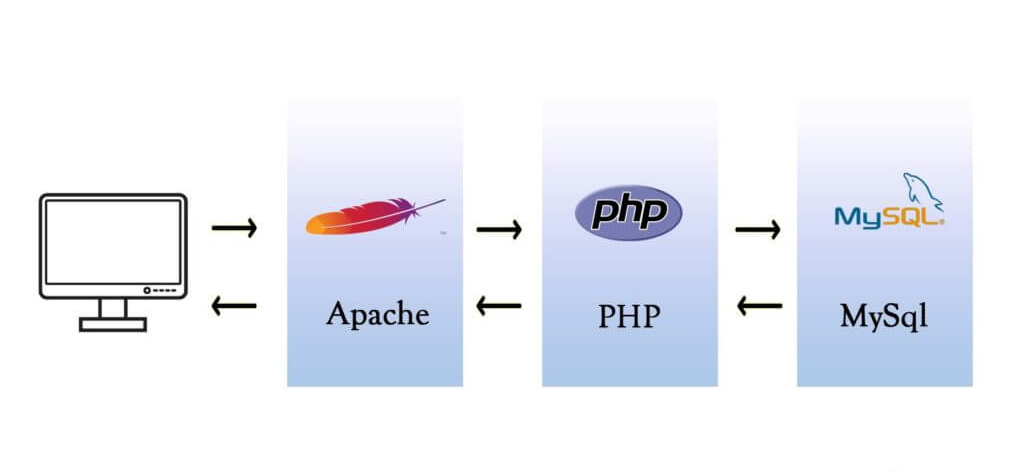
\includegraphics[width = 0.6\textwidth]{images/WAMP_LAMP.png}
    \caption{Architettura WAMP/LAMP}
\end{figure}
\newline
Per quanto riguarda i siti statici invece, una volta generato il sito è sufficiente caricare i file su qualsiasi web server o servizio di hosting, non avendo infatti la necessità di eseguire codice dinamico (es. PHP) e di interfacciarsi con un database, la struttura risultante è molto più snella. 
Avere un'architettura di questo tipo permette di ottenere delle ottimizzazioni delle prestazioni e della velocità necessaria per servire la pagina richiesta. 
\begin{figure}[h]
    \centering
    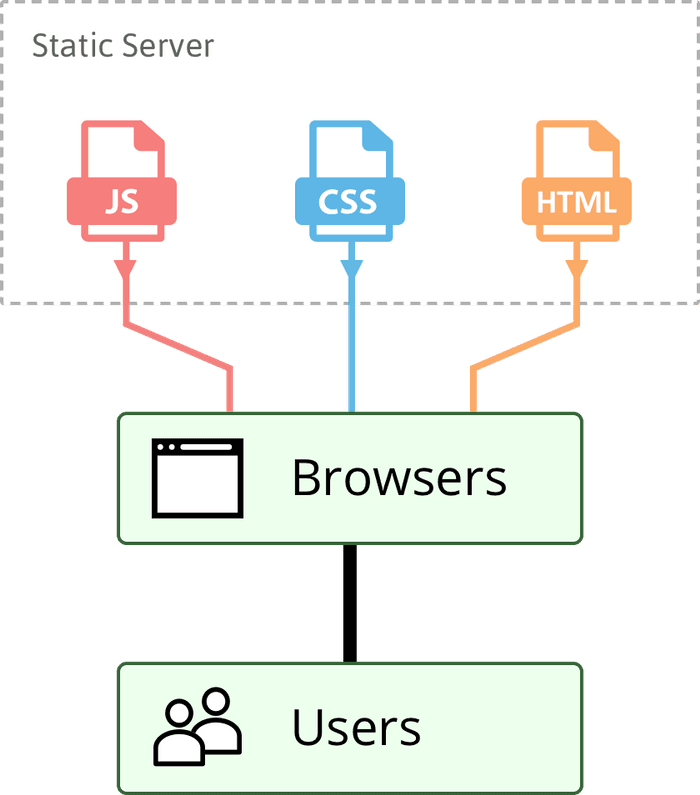
\includegraphics[width = 0.25\textwidth]{images/static.png}
    \caption{Architettura client/server SSG}
\end{figure}

%% Sezione
\section{Hugo}\label{sec:hugo}
In questa sezione verrà ripreso ed ampliato il contenuto della \cref{subsec:shugo} in quanto Hugo rappresenta l'SSG scelto per la realizzazione del caso di studio.

%% Sottosezione
\subsection{Formati supportati}
Hugo supporta una grande varietà di formati, i principali sono i seguenti:

\begin{itemize}
    \item MARKDOWN: formato di markup contenente esclusivamente il contenuto informativo, in questi file non viene definito nessun tipo di stile;
    \item HTML: formato utilizzato per definire l'organizzazione e la struttura delle pagine;
    \item CSS: formato utilizzato per definire lo stile delle pagine (es. colore, sfondo, dimensioni e tipo di carattere, ...);
    \item JavaScript: questi file vengono utilizzati principalmente per l'esecuzione di script, sono fondamentali per l'esecuzione di specifici task.
    \item JSON: vengono utilizzati per definire metadati e contenuti strutturati all'interno del sito web; 
    \item TOML, YAML: questi file vengono utilizzati per definire o aggiungere dettagli strutturali o globali del sito e delle singole pagine. 
\end{itemize}

Vengono inoltre supportati formati più specifici come reStructuredText, un formato markup utilizzato ad esempio per la documentazione tecnica, oppure AsciiDoc, anch'esso un formato markup spesso utilizzato in ambienti di sviluppo.

%% Sottosezione
\subsection{Template actions}
Le Template actions, scritte in Go Template, si riferiscono a una serie di azioni o comandi disponibili nei modelli (templates) di Hugo, che vengono utilizzati per manipolare e visualizzare i dati all'interno dei contenuti. 
Le template actions consentono di eseguire operazioni come l'iterazione attraverso gli elenchi, il controllo di flusso condizionale e l'estrazione di valori dai dati dei contenuti. Vengono utilizzate direttamente all'interno dei file HTML all'interno delle doppie graffe. \newline
Alcune delle template actions più comuni in Hugo includono:
\begin{itemize}
    \item \textbf{range}: utilizzata per iterare all'interno di un'elenco, permette ad esempio di creare dei cicli.
    \item \textbf{if, with}: consentono di aggiungere logica condizionale nei modelli. Possono essere utilizzati per visualizzare o nascondere parti del contenuto in base a condizioni specifiche;
    \item \textbf{index}: utilizzata per accedere a elementi specifici all'interno di elenchi o dizionari;
    \item \textbf{partial}: per includere modelli o contenuti da altri file. 
\end{itemize}

La \cref{img:if} mostra un'esempio di utilizzo del controllo di flusso attraverso il costrutto "if", nello specifico verifica se nei parametri che descrivono la persona è presente un'immagine: in caso positivo mostra l'immagine corrispondente altrimenti un'immagine di default.
La \cref{img:partial} mostra invece l'utilizzo della template action "partial", permettendo così di includere il file \textit{recent.html}. \newline 
Nell template actions è possibile anche selezionare specifici parametri come ad esempio \{\{ .Title \}\} che permette di inserire il titolo della pagina corrente. Allo stesso modo si può ottenere la descrizione (\{\{ .Description \}\}) o il sommario (\{\{ .Summary \}\}).

\begin{figure}[b]
    \centering
    \begin{minipage}{0.8\textwidth}
      \centering
      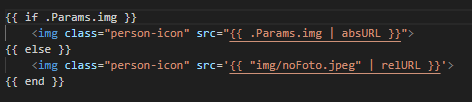
\includegraphics[width=0.8\textwidth]{images/if-template-actions.png}
      \caption{Esempio di utilizzo della template action "if"}
      \label{img:if}
    \end{minipage}
    \hspace{1cm}
    \hfill
    \begin{minipage}{0.5\textwidth}
      \centering
      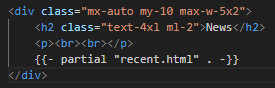
\includegraphics[width=0.8\textwidth]{images/partial-template-actions.png}
      \caption{Esempio di utilizzo della template action "partial"}
      \label{img:partial}
    \end{minipage}
\end{figure}

%% Sottosezione
\subsection{Plugin}
Hugo supporta una grande varietà di Plugin che permettono di esetendere le funzionalità di base, in questa sezione ne verranno presentati due tra i più utilizzati.
\newline 
\newline 
\textbf{{\fontsize{12}{14}\selectfont Hugo-authors}}
\newline \newline
Il plugin "hugo-authors" è progettato per semplificare la gestione dei dati degli autori. Consente di definire e visualizzare le informazioni sugli autori come nome, biografia, immagine del profilo e collegamenti ai social media, in modo più strutturato.
\newline
Per poter utilizzare questo plugin è necessario prima installarlo attraverso il modulo Hugo o includendolo nel file di configurazione (config.toml oppure config.yaml).
Successivamente è possibile creare dei nuovi autori attraverso la seguente sintassi:
\newline \newline
[author]
\newline
[[author.authors]]
\newline
name = "author name"
\newline 
bio = "author bio"
\newline 
image = "author.jpg"
\newline
social = [
\newline
\qquad    \{ name = "Twitter", link = "link" \},
\newline
\qquad    \{ name = "LinkedIn", link = "link" \}
\newline
]
\newline \newline
A questo punto è possibile associare gli autori al rispettivo contenuto specificando nel \textit{front-matter} del file markdown il nome corrispondente. Il nome svolge quindi la funzione di ID. Ad esempio:
\newline \newline
+++
\newline title = "Il mio articolo"
\newline author = "author name"
\newline 
+++
\newline \newline
Sfruttando infine le Template actions è possibile accedere alle carattersitiche dell'autore, ad esempio si può ricavare il nome scrivendo \{\{ .Params.author \}\} oppure 
applicando la stessa logica si possono ricavare le varie informazioni inserite (ad esempio la biografia).
\newline
\newline
\textbf{{\fontsize{12}{14}\selectfont Servizio delle icone social}}
\newline \newline
Questo plug-in non necessita di installazione e permette di visualizzare facilmente icone e collegamenti ai profili social. Per poterlo utilizzare bisogna aggiungere le seguenti righe di codice al file di configurazione 
\newline \newline [social]
\newline platforms = [
\newline    { name = "Twitter", icon = "twitter" },
\newline    { name = "LinkedIn", icon = "linkedin" },
\newline    { name = "GitHub", icon = "github" },
\newline    \# Altre piattaforme social
\newline ]
\newline
\newline icons = [
\newline    { name = "twitter", link = "https://example.com/twitter-icon.svg" },
\newline    { name = "linkedin", link = "https://example.com/linkedin-icon.svg" },
\newline    { name = "github", link = "https://example.com/github-icon.svg" },
\newline    \# Altre icone social
\newline ]
\newline \newline
Solo successivamente possono essere specificate all'interno della definzione degli autori (sezione precedente) o nel front matter di un contenuto.
Allo stesso modo del plugin precendente, le informazioni possono essere richiamate all'interno dei file HTML sfruttando le Template actions (in questo caso tramite \{\{ .Site.Data.social.icons \}\}).
%% Sottosezione
\subsection{Creazione del sito}\label{sec:creazione}
Dopo l'installazione di Hugo, per creare un nuovo sito è suffciente digitare da terminale il seguente comando \textbf{hugo new site NOME\_SITO}. 
In seguito a questo comando verrà costruita la struttura delle cartelle così come descritto nella \cref{subsec:shugo} che può essere modificata secondo le esigenze.
\newline
Per poter visualizzare in locale il sito che si sta creando, è necessario lanciare da terminale il comando \textbf{hugo server} oppure \textbf{npm run start} (se è stato installato npm), in seguito il sito sarà visibile all'indirizzo localhost:1313 (127.0.0.1:1313).
\newline
Altri comandi utili per la creazione del sito sono \textbf{hugo server -D} che, a differenza del comando precedente, permette di visualizzare anche i contenuti classificati come bozze ed il comando \textbf{hugo}, necessario per la costruzione del sito. Quest'ultimo comando verrà discusso nella sezione successiva.
%% Sottosezione
\subsection{Costruzione del sito}
La costruzione del sito è divisa in due fasi principali: la fase di generazione e la fase di compilazione.
\newline
\newline
\textbf{{\fontsize{12}{14}\selectfont Fase di generazione}}
\newline \newline
Il processo di generazione viene avviato attraverso il comando \textbf{hugo}, il quale genera un unico file CSS combinando i dati di file di template dei temi con eventuali fogli di stile personalizzati, unendo successivamente anche il contenuto dei file Markdown.
\newline \newline
\textbf{{\fontsize{12}{14}\selectfont Fase di compilazione}}
\newline \newline
Terminata la fase di generazione, Hugo applica i temi e genera il codice HTML e CSS per ogni pagina del sito. L'ultima fase prima di poter rendere le pagine distribuibili e visualizzabili consiste nel produrre un insieme di fogli di stile CSS, immagini e
altri file statici, ciascuno rappresentante una pagina del sito. 
Una variante più efficiente è il comando \textbf{hugo - -minify} che ottimizza il caricamento delle pagine minimizzando la dimensione dei file attraverso l'eliminazione di spazi vuoti, commenti e caratteri non necessari.
\newline
Il risulato del processo di compilazione è la creazione di due cartelle:
\begin{itemize}
    \item public: contiene il sito costruito ed è organizzata a sua volta in sottocartelle ognuna delle quali contiene una pagina singola oppure un gruppo di pagine correlate. Ogni sottocartella comprende un file HTML, i fogli di stile e i file JavaScript;
    \item resources: contiene le cache di output del processo di generazione; nello specifico, contiene risorse come immagini, file CSS, file JavaScript e altri assets statici utilizzati nel sito.
\end{itemize}
%% Sottosezione
\subsection{Hosting e distribuzione}
In seguito alla generazione e compilazione, il sito può essere caricato su qualsiasi web server o servizio di hosting. Come detto precedentemente, non è necessario eseguire elaborazioni lato server oppure richieste ad un database, pertanto è possibile utilizzare servizi di hosting completamente gratuiti.
\newline
Un'esempio di questi servizi è \textit{Github Pages}, offerto da GitHub. Quest'ultimo è uno dei servizi di hosting di repository Git più popolari al mondo che offre servizi per il controllo di versione, la collaborazione e l'hosting di progetti software (attrverso appunto Github Pages).
Alcune delle principali funzionalità di GitHub includono il controllo di versione distribuito, il tracciamento delle modifiche, la collaborazione tra sviluppatori e molto altro.
GitHub Pages è uno dei servizi offerti da Github che consente di pubblicare siti web statici direttamente da una repository GitHub, in particolare utilizza uno specifico branch chiamato "gh-pages" dal quale preleva il contenuto che viene poi pubblicato.
Di default, l'indirizzo che viene assegnato è \textit{"https://NOME\_UTENTE.github.io/NOME\_REPOSITORY/"} ma supporta anche domini personalizzati. 
\newline 
GitHub Pages tuttavia presenta dei limiti sulla dimensione dei siti che consente di hostare:
\begin{itemize}
    \item Le dimensioni della repository utilizzata per creare il sito web non deve essere superiore ad un 1GB;
    \item Le risorse messe a disposizione sono limitate a 100GB di banda e 100.000 richieste al mese;
    \item Non si dovrebbero eseguire più di dieci "build" per ora, per evitare di sovraccaricare i server e mantenerli performanti per tutti gli utenti.
\end{itemize}
I limiti appena citati possono essere superati attraverso un piano di pagamento del servizio.
\newline
Altri limiti imposti e non superabili riguardano il contenuto del sito web, GitHub infatti non consente di utilizzare questo servizio per gestire attività online e servizi di software commerciale, inoltre l'utilizzo della pagine è soggetto ai Termini di servizio di Github,
per cui sono vietati contenuti sessuali oppure violenti/minacciosi. 
%% Sottosezione
\subsection{Web Analytics}
Le web analytics sono il processo di raccolta, misurazione, analisi e reporting dei dati relativi all'uso di un sito web al fine di comprendere il comportamento degli utenti, valutare le prestazioni del sito e trarre informazioni utili per  migliorare l'esperienza degli utenti. 
Le web analytics sono fondamentali per il miglioramento dell'usabilità, l'ottimizzazione dei motori di ricerca e l'analisi delle conversioni.
\begin{itemize}
    \item \textbf{Raccolta dei Dati}: la raccolta dei dati inizia con l'implementazione di strumenti di analisi web che tracciano il comportamento degli utenti sul sito. Questi strumenti registrano dati come il numero di visite, il tempo trascorso sul sito, le pagine visitate e molto altro;
    \item \textbf{Misurazione delle Metriche Chiave}: le web analytics misurano una vasta gamma di metriche, tra cui il traffico del sito, l'origine del traffico, il tasso di rimbalzo, il tempo medio sulla pagina, le conversioni e altro ancora. Queste metriche consentono di valutare le prestazioni del sito;
    \item \textbf{Analisi dei Dati}: l'analisi dei dati comporta l'interpretazione delle metriche raccolte per comprendere i modelli e le tendenze. Ad esempio, analizzare quale fonte di traffico genera più conversioni o quali pagine del sito hanno un alto tasso di rimbalzo;
    \item \textbf{Reporting}: la creazione di report è un passaggio importante nelle web analytics. I report consentono di comunicare i risultati dell'analisi in modo chiaro e comprensibile per poter essere condivisi con i membri del team, i responsabili decisionali o i clienti;
    \item \textbf{Ottimizzazione}: le web analytics sono utilizzate per prendere decisioni sull'ottimizzazione del sito. Ciò può includere l'ottimizzazione del contenuto, delle conversioni, del carico delle pagine e altro ancora al fine di migliorare l'esperienza dell'utente e raggiungere gli obiettivi stabiliti;
    \item \textbf{Segmentazione degli Utenti}: le web analytics consentono di suddividere gli utenti in segmenti in base a criteri come la provenienza geografica, il comportamento di navigazione, il dispositivo utilizzato e altro ancora. Questa segmentazione aiuta a comprendere meglio il pubblico e a personalizzare l'esperienza dell'utente.
\end{itemize}
Uno delle più famose piattaforme di analisi web è sicuramente \textit{Google Analytics} che utilizza come strumento di analitica i cookies. 
Nel sito web che si è realizzato con questo progetto, viene utilizzata come piattafroma di analisi uno strumento meno conosciuto di Google Analytics: \textit{umami}. 
Si tratta di un'applicazione open-source compatibile con il GDPR che a differenza di Google Analytics non utilizza cookie di tracciamento ma allo stesso tempo permette di ottenere informazioni come le pagine visitate, il browser, il sistema operativo ed il dispositivo utilizzati, nonchè il paese di provenienza. Queste informazioni di base possono poi essere ampliate comprendendo ad esempio specifici eventi di interesse per l'analisi del sito web.
Umami mette inoltre a disposizione una dashboard per la presentazione del numero di visite nel corso del tempo, permettendo di visualizzare gli accessi nella giornata, nell'ultima settimana, nell'ultimo mese oppure nell'anno corrente. 
\newline 
L'utilizzo e l'implementazione di umami verranno riprese nel \cref{cap:casostudio}.


%% Capitolo  
\chapter{Realizzazione di un sito web}
%% Sottosezione
\section{Analisi dei requisiti}
Nella realizzazione di un sito web bisogna tenere in considerazione diversi aspetti che possono influenzare la buona riuscita del progetto, come ad esempio l'usabilità, l'accesibilità, l'organizzazione dei contenuti e molto altro.
Per questo motivo esistono delle linee guida e degli approcci cosolidati che permettono di creare siti web di buona qualità. Queste "best practice" si basano sull'esperienza e su ricerche condotte nel campo della progettazione web, le più comuni sono:
\begin{itemize}
    \item \textbf{Usabilità}: il sito deve essere intuitivo da utilizzare, la navigazione deve essere chiara e gli utenti dovrebbero essere in grado di trovare facilmente ciò di cui hanno bisogno;
    \item \textbf{Responsive Design}: il sito deve essere ottimizzato per dispositivi desktop, tablet e smartphone. Deve quindi adattarsi a diverse dimensioni di schermo;
    \item \textbf{Velocità di caricamento}: I siti web devono caricarsi rapidamente, riducendo al minimo il tempo di caricamento delle pagine e dele immagini;
    \item \textbf{Struttura delle informazioni}: organizzare il contenuto in modo logico utilizzando una struttura di navigazione chiara con menu, sottosezioni e collegamenti interni;
    \item \textbf{Chiarezza e semplicità}: mantienere il design pulito e senza distrazioni, l'utente dovrebbe poter comprendere facilmente il messaggio e la struttura del sito.
\end{itemize}
La loro applicazione dipenderà ovviamente dalle esigenze specifiche del sito e dal pubblico di destinazione, devono perciò essere adattate in base alle esigenze.
\newline Queste linee guida verranno poi riprese ed implementate nel \cref{cap:casostudio}.
%% Sottosezione
\section{User Experience}
Il fattore forse più importante da tenere in considerazione nella realizzazione di un sito web è l'espereinza dell'utente (UX), questo termine si riferisce a quello che prova una persona quando interagisce o immagina di interagire con un prototipo, un prodotto finito, un sistema od un servizio.
L'UX oltrepassa i limiti di altri termini come "interfaccia utente" e "usabilità" in quanto comprende tutti gli aspetti dell'esperienza che le persone hanno con i sistemi interattivi.
\newline 
Sono stati identificati tre livelli di esperienza basati sulle risorse fisiologiche e psicologiche mobilitate dall'utente durante l'interazione:
\begin{itemize}
    \item \textit{viscerale}: ricevere e interpretare gli stimoli che provengono dal mondo esterno in modo automatico ed immediato;
    \item \textit{comportamentale}: viene analizzato l'uso del sistema, la prestazione;
    \item \textit{riflessivo}: considera gli aspetti culturali e il significato dell'uso di un prodotto.
\end{itemize}
L'esperienza dell'utente ha inizio prima dell'effettivo utilizzo, in quanto una tecnologia, o l'immagine che vediamo di essa, può incuriosire, emozionare ed indurre risposte “viscerali”, lasciando immaginare le cose che faremmo avendola a nostra disposizione.
Durante l'interazione si possono identificare la soddisfazione dell'utente, ovvero il grado con cui gli utenti giudicano quanto le tecnologie incontrano le loro esigenze, e la piacevolezza, considerata una componente rilevante della soddisfazione e provata dalle persone durante l'uso di un prodotto.
Quest'ultima non è legata a a termini funzionali ma all'esperienza sensoriale e le emozioni positive suscitate. 
\newline
La user experience è ormai diventata una condizione necessaria per la sopravvivenza e la crescita di qualsiasi prodotto o servizio, una UX insoddisfacente può portare ad un calo dei guadagni e della visibilità generale.
%% Sottosezione
\section{Scelta del tema}
La scelta di un tema è una decisione importante nel processo di sviluppo di un sito web, la cui scelta dipende ovviamente del tipo di progetto che si sta realizzando. 
La sua importanza non è dovuta solo all'aspetto visivo ma soprattutto all'organizzazione dei contenuti e alle funzionalità che offre.
\newline
Hugo mette a disposizione sul sito ufficiale una grande varietà di temi suddivisi in categorie (Blog, Company, Minimal, ...) che facilitano quindi la scelta in base a ciò che si vuole realizzare. 
Inoltre per la maggior parte dei temi è possibile provare una demo che permette di visualizzare l'aspetto generale e navigare nelle varie sezioni in modo da poterne analizzare la struttura. Sono poi generalamente presenti la documentazione del tema stesso, le specifiche per scaricarlo, il collegamento alla repository di GitHub
ed informazioni più specifiche come la versione di Hugo necessaria per eseguire il tema e l'ultimo aggiornamneto disponibile.
\newline
In seguito alla procedura di installazione, avendo a disposizione i file sorgenti, è possibile modificare il comportamento o aggiungere funzionalità al tema scelto. Allo stesso modo, se nessun tema soddisfa le esigenze richieste, è possibile creare un tema partendo da zero, per farlo si deve creare una sottocartella \textit{layouts} all'interno della directory \textit{themes}
e caricare al suo interno i vari file HTML, CSS e JS.
\subsection{Tipologie di temi}
Un'altra distinzione degna di nota in Hugo riguarda la possibilità di installare "temi standard" e "temi non standard". I primi si riferiscono ai temi precdentemente descritti mentre i secondi sono più complessi in quanto offrono delle funzionalità e dell'estetica superiore, rendendo necessariamnete più complesso e costoso lo sviluppo ed il mantenimento.
\newline \newline
\textbf{{\fontsize{12}{14}\selectfont Installazione temi standard}}
\newline \newline
La configurazione di un tema standard è relativamente semplice, una volta inizializzato un nuovo sito (così come descritto nella \cref{sec:creazione}), il nuovo tema va scaricato seguendo le istruzioni all'interno della cartella \textit{themes}. 
A questo punto l'ultimo passaggio è collegare il sito creato con il tema appena scaricato, per farlo è necessario modificare il file di configurazione (config.toml oppure config.yml) aggiungendo la riga \textbf{theme="NOME\_TEMA"}.
\newline
Se successivamente si desidera cambiare il tema, è necessario scaricarlo all'interno della stessa cartella del precedente e modificare il nome nel file di configurazione (NB: i temi possono coesistere all'interno della cartella \textit{themes}, non è necessario cancellare il precedente).
\newline \newline
\textbf{{\fontsize{12}{14}\selectfont Installazione temi non standard}}
\newline \newline
I temi non standard modificano significativamente la struttura dei siti in cui vengono utilizzati, generalmente hanno più file di configurazione e modificano anche altre cartelle (ad esempio la cartella \textit{content}) e per questo necessitano la creazione di altre cartelle per il salvataggio di determinati contenuti.
%% Capitolo  
\chapter{Caso di studio}\label{cap:casostudio}

%% Capitolo  
\chapter{Conclusioni}

%% Fine dei capitoli normali, inizio dei capitoli-appendice (opzionali)
\appendix

%\part{Appendici}

\chapter{Glossario}


%% Parte conclusiva del documento; tipicamente per riassunto, bibliografia e/o indice analitico.
\backmatter

%% Riassunto (opzionale)
%\summary
%Maecenas tempor elit sed arcu commodo, dapibus sagittis leo egestas. Praesent at ultrices urna. Integer et nibh in augue mollis facilisis sit amet eget magna. Fusce at porttitor sapien. Phasellus imperdiet, felis et molestie vulputate, mauris sapien tincidunt justo, in lacinia velit nisi nec ipsum. Duis elementum pharetra lorem, ut pellentesque nulla congue et. Sed eu venenatis tellus, pharetra cursus felis. Sed et luctus nunc. Aenean commodo, neque a aliquam bibendum, mauris augue fringilla justo, et scelerisque odio mi sit amet diam. Nulla at placerat nibh, nec rutrum urna. Donec ut egestas magna. Aliquam erat volutpat. Phasellus vestibulum justo sed purus mattis, vitae lacinia magna viverra. Nulla rutrum diam dui, vel semper mi mattis ac. Vestibulum ante ipsum primis in faucibus orci luctus et ultrices posuere cubilia Curae; Donec id vestibulum lectus, eget tristique est.

%% Bibliografia (praticamente obbligatoria)
\bibliographystyle{plain_\languagename}%% Carica l'omonimo file .bst, dove \languagename ? la lingua attiva.
%% Nel caso in cui si usi un file .bib (consigliato)
\bibliography{thud}
%% Nel caso di bibliografia manuale, usare l'environment thebibliography.

%% Per l'indice analitico, usare il pacchetto makeidx (o analogo).

\end{document}